\documentclass[a4paper, 12pt]{article}
\usepackage{CJKutf8}
\usepackage{graphicx}

\title{analyze 'ioqueue' in pjsip}
\author{icefreedom}
\date{\today}

\begin{document}

\maketitle

\begin{CJK}{UTF8}{gkai}

\section{Introduction}
ioqueue是pjsip中的异步网络通讯的模块, 与timer的机制很类似, 在一个线程中循环调用poll来处理多路网络IO.

\section{System Calls}
select, poll, epoll
\begin{description}
\item[select]
它的作用是等待fd\_set中的一个变为ready, 定义如下:
int select(int nfds, fd\_set *readfds, fd\_set *writefds,
           fd\_set *exceptfds, struct timeval *timeout);
	@param nfds readfds, writefds,  exceptfds中的fd最大值, 加上1
	要注意的是调用select之后readfds, writefds和exceptfds可能会被修改, 因此下次调用需要重置。
	在unix较老就已经支持该接口, 但它不能超过系统能同时打开的最大fd数。
 \item[poll]
它的作用同select, 但它是unix后来才加入的接口, 定义如下:
int poll(struct pollfd *fds, nfds\_t nfds, int timeout);
	@fds 相当于select中的readfds, writefds, exceptfds的集合
	它没有最大fd数的限制
\item[epoll]
epoll也是后来才加入的接口, 它改进了select和poll的效率, 因为select, poll都是遍历fd\_set来看监听每个事件,它们会随着fd数的
增加而效率降低, 而epoll则不是去遍历每个fd. 定义如下:
 int epoll\_create(int size);  创建epoll, 打开了一个fd;
int epoll\_ctl(int epfd, int op, int fd, struct epoll\_event *event); 注册要监听的fd
int epoll\_wait(int epfd, struct epoll\_event * events, int maxevents, int timeout); 等待事件ready
\end{description}

\section{Data Structure}
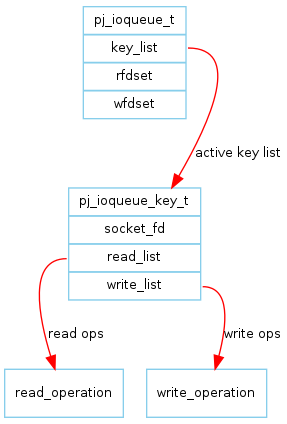
\includegraphics[width=\textwidth]{ioqueue.png}

\section{Flow}
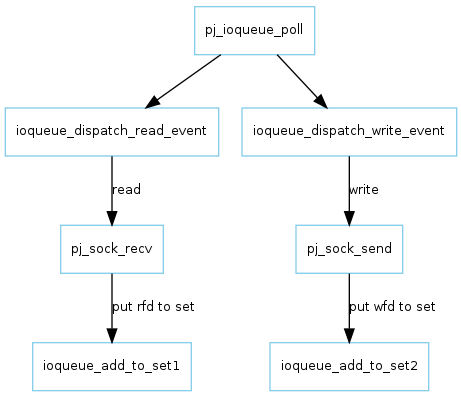
\includegraphics[width=\textwidth]{ioqueue_flow.png}


\end{CJK}
\end{document}




